\documentclass[UTF8,zihao=-4]{ctexart}
\usepackage[a4paper,margin=2.5cm]{geometry}
\usepackage{amsmath, amssymb, amsthm}
\usepackage{bm}
\usepackage{hyperref}
\usepackage{graphicx}
\usepackage{caption}
\usepackage{listings}
\usepackage{xcolor}
\usepackage{float}
\usepackage{booktabs}
\usepackage{longtable}
\usepackage{multirow}
\usepackage{placeins}
\graphicspath{{figures/}}

% 代码样式
\lstdefinestyle{code}{
  basicstyle=\ttfamily\small,
  numbers=left,
  numberstyle=\tiny,
  numbersep=8pt,
  keywordstyle=\color{blue},
  commentstyle=\color{teal!70!black},
  stringstyle=\color{orange!70!black},
  showstringspaces=false,
  breaklines=true,
  frame=single,
  framerule=0.3pt,
  rulecolor=\color{black!15}
}
\lstset{style=code}

\title{多模态大模型前沿:跨模态理解、融合与适配器设计}
\author{}
\date{\today}

\begin{document}
\maketitle

\section{文本 + 图像:CLIP、BLIP、GPT-4V}
\subsection{体系概览}
在“文本+图像”场景中,模型需要同时理解视觉内容与语言语义,常见架构如图\ref{fig:multimodal_pipeline_cn} 所示:各模态先经独立编码器提取特征,再通过跨模态融合层对齐,最终交由语言解码器生成响应。
\begin{figure}[H]
  \centering
  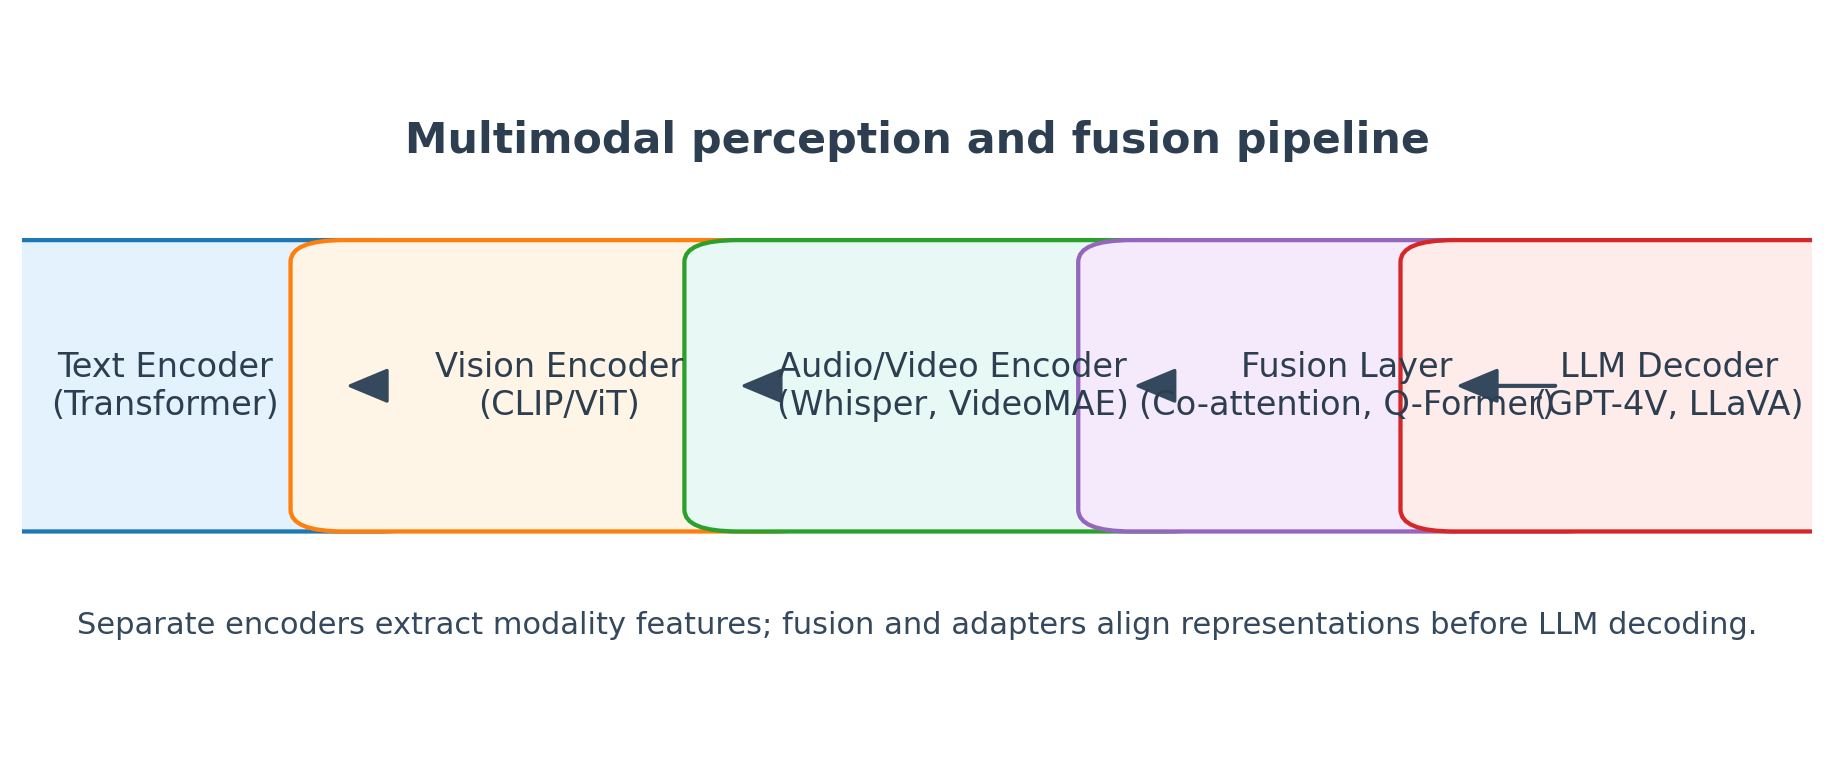
\includegraphics[width=0.95\textwidth]{multimodal_pipeline.png}
  \caption{多模态感知与融合流水线:文本、图像、音频编码后输入融合层,最后由 LLM 解码。}
  \label{fig:multimodal_pipeline_cn}
\end{figure}

\subsection{CLIP:对比学习的跨模态对齐}
\begin{itemize}
  \item \textbf{编码器结构:} 文本编码器(Transformer)与图像编码器(ViT/ResNet),分别输出归一化向量;
  \item \textbf{训练目标:} InfoNCE 对比损失,最大化配对文本-图像余弦相似度,最小化非配对样本;
  \item \textbf{应用:} 零样本分类、图文检索、提示工程(CLIP 引导扩散模型生成)。
\end{itemize}
CLIP 的成功表明,统一的对比学习空间能够支撑强大的跨模态理解能力。

\subsection{BLIP/BLIP-2:生成式对齐}
\begin{itemize}
  \item \textbf{BLIP:} 采用 Vision Transformer + Q-Former 模块,将图像特征转换为语言查询 token,与 BERT 解码器交互;
  \item \textbf{BLIP-2:} 引入 frozen LLM(如 Flan-T5、OPT),通过 Q-Former 生成少量视觉 token 作为软提示,大幅降低训练成本;
  \item \textbf{能力:} 支持图像描述、图文问答、多轮对话。
\end{itemize}

\subsection{GPT-4V 与开放式多模态模型(LLaVA, MiniGPT-4)}
\begin{itemize}
  \item \textbf{GPT-4V:} 多模态输入接口,模型具备 OCR、图表理解、视觉推理能力,强调安全与拒绝策略;
  \item \textbf{LLaVA:} 将 CLIP/ViT 特征映射到 LLaMA 词嵌入空间,通过监督微调实现图文对话;
  \item \textbf{MiniGPT-4:} 利用 BLIP-2 Q-Former + Vicuna,采用视觉描述+语言微调构造指令数据。
\end{itemize}

\section{文本 + 音频 / 视频 / 传感器融合}
\subsection{音频融合}
\begin{itemize}
  \item \textbf{音频编码器:} Whisper、wav2vec 2.0、HuBERT;输出帧级或句级表征;
  \item \textbf{任务:} 语音识别、语音翻译、语音问答、音乐描述;
  \item \textbf{多模检索:} 通过对比学习对齐文本和音频嵌入,实现“描述找音频”或“哼唱找歌”。
\end{itemize}

\subsection{视频融合}
\begin{itemize}
  \item \textbf{时序编码:} VideoMAE、TimeSformer、Timesformer-CLIP,将视频切分为帧 token;
  \item \textbf{跨模态桥接:} 使用时序注意力或 LSTM 将视频特征发送到语言模型;
  \item \textbf{任务案例:} 视频字幕生成(Video Captioning)、时序问答(VideoQA)、行为识别;
  \item \textbf{长视频处理:} 结合关键帧抽取、层次化记忆、检索增强(Video-RAG)。
\end{itemize}

\subsection{传感器数据融合}
\begin{itemize}
  \item \textbf{模态类型:} 陀螺仪、加速度计、雷达、LiDAR、温度/湿度等;
  \item \textbf{编码方式:} Transformer/TCN,或通过离散化/谱分析转换为 token 序列;
  \item \textbf{应用场景:} 自动驾驶(多传感器感知)、工业 IoT(异常检测)、医疗监测(生理信号解释);
  \item \textbf{挑战:} 采样率差异大、噪声多、标注稀缺,需要自监督预训练与跨模态对齐。
\end{itemize}

\section{多模态输入的对齐与适配器设计}
\subsection{对齐技术谱系}
图\ref{fig:alignment_adapters_cn} 总结了常见对齐模块:投影头将不同模态映射到共享潜空间,跨模态适配器负责信息交互,任务头针对下游目标优化。
\begin{figure}[H]
  \centering
  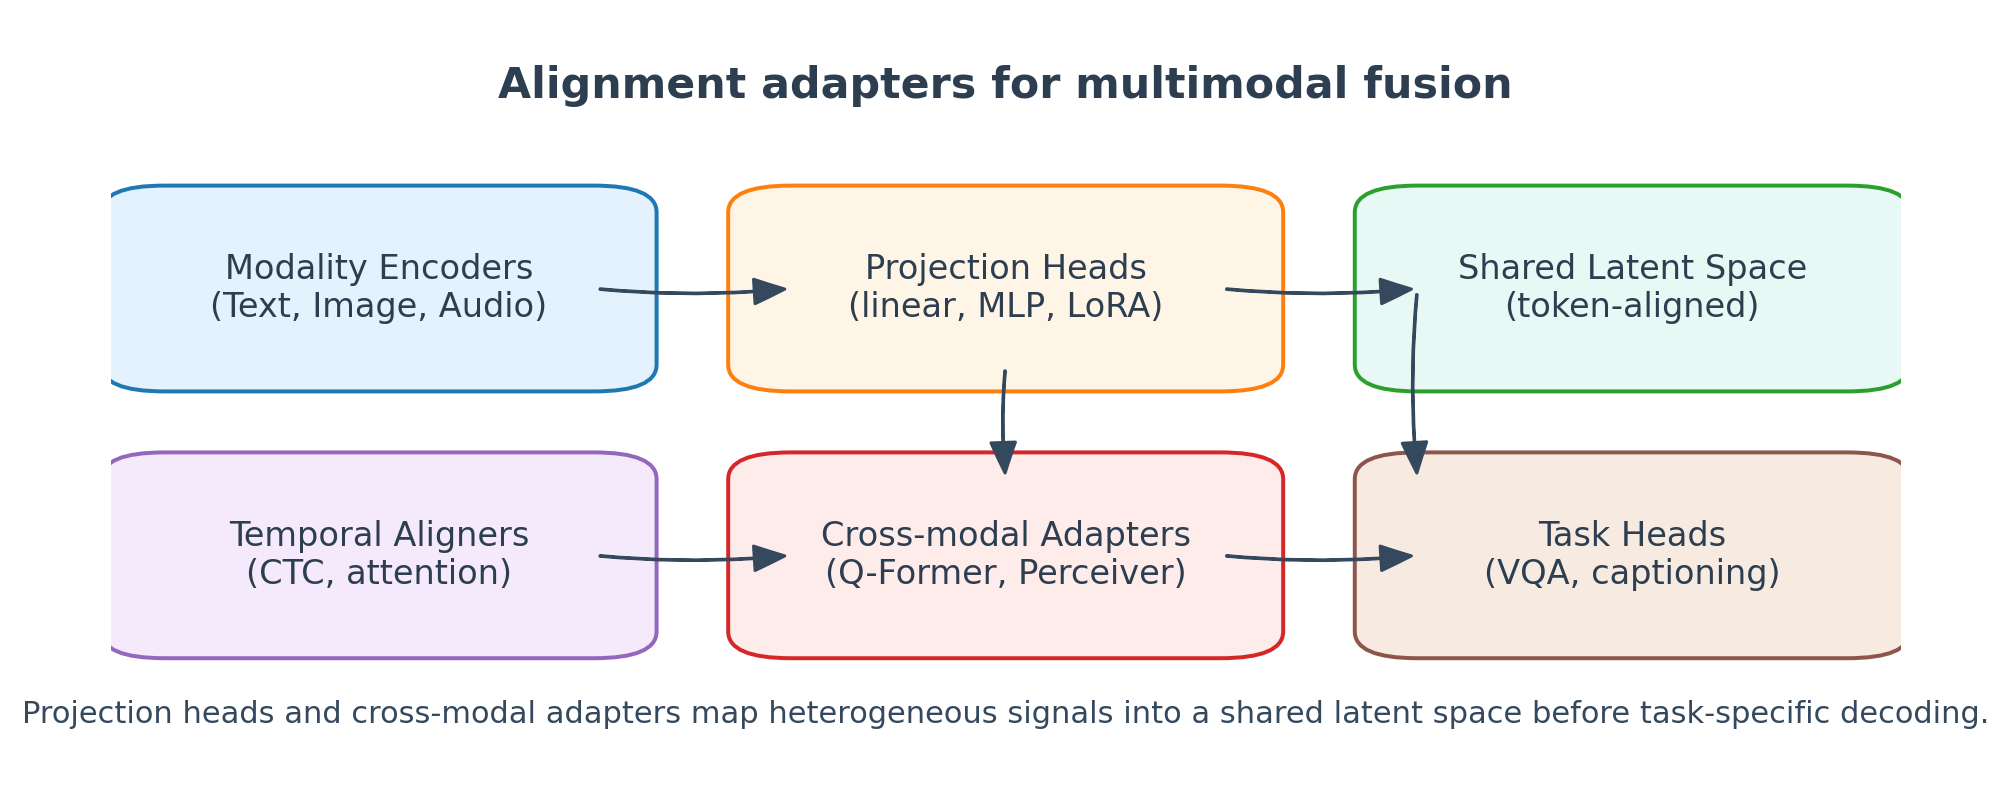
\includegraphics[width=0.95\textwidth]{alignment_adapters.png}
  \caption{多模态对齐与适配器:投影头、跨模态适配器、任务头协同实现特征融合。}
  \label{fig:alignment_adapters_cn}
\end{figure}

\subsection{投影与映射}
\begin{itemize}
  \item \textbf{线性/MLP 投影:} 简单高效,适合特征维度相近的模态;
  \item \textbf{LoRA/Adapter:} 在冻结主干模型的情况下,通过低秩更新或瓶颈结构完成跨模态对齐;
  \item \textbf{Prompt Tuning:} 以虚拟 token 形式在语言模型中注入视觉/音频信息。
\end{itemize}

\subsection{跨模态适配器}
\begin{itemize}
  \item \textbf{Q-Former:} 将视觉特征压缩为固定长度的查询 token,与 LLM 交互;
  \item \textbf{Perceiver / PerceiverIO:} 使用交叉注意力处理任意模态,支持可变长度输入;
  \item \textbf{Token-merging/动态采样:} 在长视频/音频中选择关键片段,降低计算量。
\end{itemize}

\subsection{对齐目标与训练策略}
\begin{itemize}
  \item \textbf{对比损失:} CLIP 式的 InfoNCE、Triplet Loss;
  \item \textbf{掩码预测:} Masked Multi-modal Modeling(如 BEiT-3);
  \item \textbf{指令微调:} 构造跨模态指令数据(文本描述 + 图像/音频/视频),进行监督微调;
  \item \textbf{检索增强:} 结合多模态向量库,触发 RAG 工作流,提供外部知识。
\end{itemize}

\subsection{案例:LLaVA 微调流程}
\begin{enumerate}
  \item 使用 CLIP ViT-L/14 提取图像特征;
  \item 通过线性层映射到 LLaMA 词向量空间;
  \item 构造多模态指令数据集(约 150K 对话轮次)进行监督微调;
  \item 在下游任务(VQA、图像描述)上评估并采用 Self-Instruct 扩充数据。
\end{enumerate}

\section*{实践建议}
\begin{itemize}
  \item 在数据层面对不同模态进行质量校验与时间对齐,减少噪声干扰;
  \item 采用模块化适配器(如 LoRA)避免对大模型进行全量调参,降低计算成本;
  \item 引入安全与偏见评估(如图像误判、音频识别偏差),建立人工审核机制;
  \item 结合多模态 RAG 和工具调用扩展模型能力,实现检索-推理闭环。
\end{itemize}

\section*{参考文献}
\begin{itemize}
  \item Radford et al. ``Learning Transferable Visual Models From Natural Language Supervision.'' ICML, 2021.
  \item Li et al. ``BLIP-2: Bootstrapping Language-Image Pre-training with Frozen Image Encoders and Large Language Models.'' ICML, 2023.
  \item OpenAI. ``GPT-4V(ision) System Card.'' Technical Report, 2023.
  \item Alayrac et al. ``Flamingo: a Visual Language Model for Few-Shot Learning.'' NeurIPS, 2022.
  \item Bai et al. ``Q-Former: Querying Transformer for Multi-modal Interaction.'' arXiv, 2023.
\end{itemize}

\end{document}

